%%%%%%%%%%%%%%%%%%%%%%%%%%% asme2ej.tex %%%%%%%%%%%%%%%%%%%%%%%%%%%%%%%
% Template for producing ASME-format journal articles using LaTeX    %
% Written by   Harry H. Cheng, Professor and Director                %
%              Integration Engineering Laboratory                    %
%              Department of Mechanical and Aeronautical Engineering %
%              University of California                              %
%              Davis, CA 95616                                       %
%              Tel: (530) 752-5020 (office)                          %
%                   (530) 752-1028 (lab)                             %
%              Fax: (530) 752-4158                                   %
%              Email: hhcheng@ucdavis.edu                            %
%              WWW:   http://iel.ucdavis.edu/people/cheng.html       %
%              May 7, 1994                                           %
% Modified: February 16, 2001 by Harry H. Cheng                      %
% Modified: January  01, 2003 by Geoffrey R. Shiflett                %
% Use at your own risk, send complaints to /dev/null                 %
%%%%%%%%%%%%%%%%%%%%%%%%%%%%%%%%%%%%%%%%%%%%%%%%%%%%%%%%%%%%%%%%%%%%%%

%%% use twocolumn and 10pt options with the asme2ej format
\documentclass[twocolumn,10pt]{asme2ej}

\usepackage{epsfig} %% for loading postscript figures
\usepackage[T1]{fontenc}
\usepackage{lipsum}% http://ctan.org/pkg/lipsum
\usepackage{graphicx}% http://ctan.org/pkg/graphicx
% ....


%% The class has several options
%  onecolumn/twocolumn - format for one or two columns per page
%  10pt/11pt/12pt - use 10, 11, or 12 point font
%  oneside/twoside - format for oneside/twosided printing
%  final/draft - format for final/draft copy
%  cleanfoot - take out copyright info in footer leave page number
%  cleanhead - take out the conference banner on the title page
%  titlepage/notitlepage - put in titlepage or leave out titlepage
%  
%% The default is oneside, onecolumn, 10pt, final


\title{Caccia al tweet: un approccio per la geolocalizzazione di un utente sulla base dei suoi tweet}

%%% first author
\author{Valerio Gregori
    \affiliation{
    Email: val.gregori2@stud.uniroma3.it
    }	
}

%%% second author
%%% remove the following entry for single author papers
%%% add more entries for additional authors
\author{Mattia Iodice
    \affiliation{ 
        Email: mat.iodice1@stud.uniroma3.it
    }
}

%%% third author
%%% remove the following entry for single author papers
%%% add more entries for additional authors
\author{Alessandro Oddi
    \affiliation{
        Email: ale.oddi1@stud.uniroma3.it
    }
}


\begin{document}

\maketitle    


%%%%%%%%%%%%%%%%%%%%%%%%%%%%%%%%%%%%%%%%%%%%%%%%%%%%%%%%%%%%%%%%%%%%%%
\begin{abstract}
{\it Nella relazione  viene presentata l'implementazione di un framework per la geolocalizzazione di un utente a partire dal corpus dei suoi tweet. L'obiettivo prefissato era appunto l'implementazione del processo di geolocalizzazione, basato sull'articolo  \textit{You are where you tweet} di Cheng, Caverlee e Lee, prendendo spunto dal lavoro dello studente F. Tanzi.  Il documento \'e strutturato in sezioni, ciascuna focalizzata su un aspetto diverso del lavoro svolto.  In particolare, dopo una breve descrizione delle caratteristiche fondamentali degli strumenti utilizzati, vengono descritti gli approcci seguiti nella fase di implementazione, insieme alla giustificazione delle scelte architetturali e alle motivazioni che hanno spinto alla reimplementazione totale del tool. Nella sezione finale vengono quindi presentati i risultati ottenuti, fornendo un confronto diretto con le metriche riportate nell'articolo precedentemente citato. }
\end{abstract}


%%%%%%%%%%%%%%%%%%%%%%%%%%%%%%%%%%%%%%%%%%%%%%%%%%%%%%%%%%%%%%%%%%%%%%
\section{Dataset di riferimento}


La prima parte del lavoro svolto ha riguardato lo studio dell'articolo \textit{You are where you tweet}  insieme all'analisi dei dati in esso utilizzati.
Vengono quindi presentati i punti salienti emersi dall'indagine.\\
I dati presi in analisi nello studio condotto fanno riferimento a un dataset relativo a un insieme di tweet estrapolati e suddivisi in training set e test set. In particolare, le caratterisitche fondamentali sono le seguenti:
\begin{enumerate}

\item  il processo di estrazione dei tweet \'e avvenuto tra il Settembre del 2009 al Gennaio del 2010

\item il training set contiene $115,886$ utenti di Twitter e $3,844,612$ aggiornamenti da parte degli utenti stessi. 

\item ciascuna localit\'a degli utenti \'e automaticamente etichettata negli USA con livello di dettaglio relativo alla citt\'a.

\item il test set contiene $5,136$ utenti di Twitter e $5,156,047$ tweets

\item tutte le localizzazioni degli utenti sono ottenute dalla posizione dei loro telefoni e sono espresse nella forma \textit{latitudine,longitudine}.
\end{enumerate}


Considerate le dimensioni piuttosto contenute dei dati in questione, in un primo momento abbiamo definito un modulo per arricchire (locupletare) il dataset. La scelta \'e stata guidata inoltre dall'esigenza di rispondere in modo efficiente ed efficace all'evoluzione della lingua. Infatti, le formule di espressione linguistiche, in contesti estremamente dinamici come quelli dei social network, sono soggette a continui cambiamenti: i.e. slang, neologismi, trand sociali ecc.
\begin{figure} 
\centerline{\psfig{figure=figure/twettami.png,width=3.30in}}
\caption{Architettura del modulo per il retrieve di tweet dallo stream. Vengono scartate citt\'a non USA e vengono associati agli stati alle citt\'a non correttamente formattate.}
\label{gazproc.ps}
\end{figure}


 
Il modulo implementato \'e essenzialmente un filtro che sfrutta lo stream offerto da \textbf{Twitter4j} effettuando una cernita tra tweet di interesse e non.\\ Per tweet di interesse si fa riferimento alla classe di aggiornamenti provenienti da utenti \textit{ben geolocalizzati}: l'attributo \textit{position} dell'utente deve comparire nella forma \textit{citt\'a , stato} e la coppia in questione deve essere collocabile all'interno del territorio statunitense. Inoltre per far fronte all'eccessivo numero di utenti che  dichiarano la citt\'a senza fornire lo Stato di appartenenza si \'e deciso di seguire un approccio gazetteer per l'individuazione dello Stato.\\ Considerando l'ingente tasso di omonimia fra i nomi delle citt\'a americane, data una citt\'a senzo uno stato, si associa ad essa lo Stato relativo alla citt\'a pi\'u popolosa con quel nome. \\Mediante l'utilizzo di questo approccio vengono scartati fino all' $80\%$ di tweet che non sono geotaggati. 


\section{Problematiche  iniziali}

L'obiettivo definito all'inizio del progetto era improntato all' \textit{intention mining} degli utenti, diversificandoli sulla base della loro localizzazione. \\ Per il task di localizzazione si voleva utilizzare il tool realizzato dallo studente Tanzi e quindi si \'e proceduto con un'attenta analisi del codice e delle rispettive funzionalit\'a.
Gi\'a dalla prima esecuzione non \'e stato possibile ottenere l'output sperato. \\In particolar modo, \'e emerso che il dataset in input prensentava tweet malformattati che non rispettavano la struttura necessaria per l'esecuzione del tool. \\ Escludendo i tweet in questione e testando il tool su un sottoinsieme del dataset iniziale \'e stato quindi possibile effettuare una stima del tempo d'esecuzione del processo di \textit{parsing} sull'intero dataset. Il tempo richiesto stimato ammontava a circa una settimana a causa dell'utilizzo di strumenti non strettamente necessari, come spiegato nella Sezione successiva.  \\ Risolti quindi i principali problemi legati ai tempi di computazione, si \'e proceduto con l'esecuzione del processo di geolocalizzazione. Anche qui, purtroppo, i costi d'esecuzione non sono stati soddisfacenti: l'implementazione aveva un costo pari a $O(n^3)$, con tempi di esecuzione stimati di circa 6 giorni.\\ Alla luce delle problematiche riscontrate si \'e quindi deciso di rinunciare al task legato all'intention mining degli utenti e piuttosto di focalizzarsi su un'implementazione funzionante e performante del processo di geolocalizzazione.

\section{Descrizione dei flussi di esecuzione}


Con l'intento di ridefinire l'intero processo di geolocalizzazione, sono stati definiti tre macro-procecessi:
\begin{enumerate}
\item Parsing
\item Calcolo del Tf-Idf
\item Validazione
\end{enumerate}   

Nel paper \textit{You Are Where You Tweet} il fulcro del processo di geolocalizzazione dell'utente \'e l'utilizzo di un indice \textbf{tf-idf} sulle parole utilizzate all'interno dei tweet analizzati. Un requisito fondamentale per la costruzione di un tf-idf di qualit\'a risiede nella qualit\'a del training set. A tal fine, \'e stato creato un package dedicato al raffinamento e alla pulizia dei dati. 


%\begin{table}[t]
%\caption{In tabella il confronto tra YAGO e Freebase in termini di fatti ed entit\'a presenti}
%\begin{center}
%\label{table_ASME}
%\begin{tabular}{c l l}
%& & \\ % put some space after the caption
%\hline
%Knowledge Graph & \# Fatti & \# Entit\'a \\
%\hline
%YAGO & 120 M & \ 10 M \\
%Freebase & 2.4 B & \ 44 M \\
%\hline
%%\end{tabular}
%\end{center}
%\end{table}

Nell'utilizzare YAGO viene consigliato di usare il core dello stesso knowledge graph, perci\'o il processo \'e implementato sui file descritti in precedenza, che rappresentano proprio il nucleo del grafo. Abbiamo comunque ritenuto opportuno analizzare i dati presenti e abbiamo estratto diverse  informazioni. \\Dal file yagoFacts.tsv emerge che i fatti presenti sono \textbf{5.625.089}, mentre da yagoTransitiveTypes.tsv sono invece state contate \textbf{5.129.147} entit\'a. Il dato che emerge \'e che si tratta di un grafo poco denso, in cui i nodi che hanno almeno un arco entrante o uno uscente sono \textbf{2.632.727}.
\\ Un ulteriore aspetto interessante che abbiamo notato nell'analisi dei documenti messi a disposizione \'e che delle \textbf{100} relazioni attestate, solo \textbf{37} compaiono nei fatti presenti in \textit{yagofacts}.
\section{Implementazione di Lector}

I dati riportati fanno riferimento all'esecuzione su un pc con le seguenti specifiche:
\begin{enumerate}
\item Intel Core i7-6700HQ
\item memoria fisica installata 8.00GB
\item SSD
\end{enumerate}


\subsection{Rimozione rumore e frasi non relazionali}

Il processo di estrazione di fatti \'e stato implementato in Java, sebbene alcuni passaggi fondamentali siano stati sviluppati con l'ausilio di strumenti supplementari come MySQL e script bash. \\Analizzando il file annotato \textit{sentences\_all.tsv} sono emerse alcune frasi particolari e problematiche per alcuni aspetti implementativi: si tratta di frasi spropositatamente lunghe e senza alcun significato, per lo pi\'u costituite da sequenze di entit\'a. \textit{Abbiamo quindi filtrato il file escludendo le frasi pi\'u lunghe di 1500 caratteri}. Seguendo i passaggi fondamentali del processo seguito da Lector abbiamo poi trasformato ciascuna frase in una sequenza di triple, costituite da frasi racchiuse tra due entit\'a consecutive.
\begin{figure} 
\centerline{\psfig{figure=figure/sbo.png,width=3.20in}}
\caption{Prefiltraggio del dump di Wikipedia}
\label{step1.ps}
\end{figure}
\\Ciascuna tripla \'e stata quindi data in pasto ad un filtro relazionale, con l'obiettivo di scartare tutte le frasi che non fossero relazionali,  come mostrato in Figura 2. Il file ottenuto in output conteneva \textbf{7.631.515} triple distinte, e perci\'o ne consegue che  il filtro ha scartato circa \textbf{l'85\%} delle triple. Di queste \textbf{7.631.515} abbiamo contato quelle con soggetto e oggetto entrambi presenti nelle entit\'a definite in yagoTypes: \textbf{5.480.597} triple.  A questo punto abbiamo deciso di procedere attraverso quattro esecuzioni parallele: 

\begin{enumerate}
\item la prima senza considerare n\'e frasi lista n\'e generalizzazione
\item la seconda effettuando la \textbf{generalizzazione} di alcune categorie di termini ricorrenti (lavori, numeri, stati, nazionalit\'a)
\item la terza effettuando la \textbf{generalizzazione} parallelamente ad un pesante processo di \textbf{stopping}
\item la quarta, pi\'u che altro complementare alle  precedenti, \textbf{normalizzando liste} di entit\'a
\end{enumerate}

Tale scelta  ci ha consentito di valutare singolarmente i quattro approcci descritti, permettendoci poi di trarre conclusioni sull'effettivo beneficio apportato.

\subsection{Associazione di frasi e relazioni senza stopping e generalizzazione}

Nella prima fase si \'e quindi direttamente proceduto con l'associazione di frasi alle relazioni. Dovendo confrontare soggetto e oggetto di 7 milioni di triple con soggetto e oggetto di 5 milioni di fatti, abbiamo intuito che una  buona soluzione in termini di efficienza e soprattutto di flessibilit\'a  potesse derivare dall'utilizzo di un DBMS. Infatti la logica SQL si presta particolarmente bene alle operazioni descritte nel paper: l'associazione di frasi alle relazioni non \'e altro che un join tra soggetto  e oggetto di una tripla con soggetto e oggetto nei fatti presenti in YAGO. Abbiamo quindi innanzitutto definito la tabella \textit{yagoFacts}(\underline{sub},\underline{relation},\underline{ob}), nella quale abbiamo importato i fatti dal .tsv yagoFacts. A questo punto per ciascuna tripla presente \'e stato sufficiente eseguire una query del tipo: \\
\begin{equation}
\small{\small{\textit{SELECT * FROM yagoFacts WHERE sub=subjT AND ob=objT}}}
\end{equation}
In questa fase \'e stato interessante osservare che:

\begin{enumerate}
\item le query che hanno restituito almeno un match sono state \textbf{475.062}. Questo dato \'e risultato particolarmente  rilevante perch\'e, se sottratto al numero di triple che hanno soggetto e oggetto entrambi appartenenti alle entit\'a di YAGO\footnote{5.480.597}, indica il massimo numero di fatti estraibili: poco pi\'u di \textbf{5 milioni}.
\item ogni query restituisce un certo numero di relazioni, quelle appunto gi\'a esistenti tra soggetto e oggetto all'interno di YAGO. \'E emerso che la somma delle relazioni restituite \'e \textbf{547.601}. Ci\'o indica che, in media, pero ogni coppia soggetto-oggetto ci sono \textbf{1.15} fatti.
\item il numero di frasi univoche  presenti in \textit{relPhraseCount} \footnote{Vedi 2.3 per definizione} \'e circa \textbf{85.000}, mentre le tuple presenti sono \textbf{111.514}  
\end{enumerate}

\begin{figure} 
\centerline{\psfig{figure=figure/join1.png,width=3.60in}}
\caption{Join tra le triple e i fatti}
\label{step1.ps}
\end{figure}

L'esecuzione di questo join ha richiesto circa 120 minuti.

\subsection{Misurazione della forza  di un'associazione entit\'a-frase}
La tabella \textit{relPhraseCount} mette appunto in relazione ciascuna relazione con un certo numero di frasi e il numero di occorrenze. Per misurare quindi la forza dell'associazione tra relazione e frase abbiamo riutilizzato la formula proposta in Lector:
\begin{equation}
P(r_i|p) =  \frac{c(p,r_i)}{\sum_{j\in{R}}c(p,r_j)}
\end{equation}
Abbiamo quindi definito la nuova tabella \textit{relPhraseScore(\underline{rel},p\underline{hrase},score,probability)}, in cui inserire, appunto i valori di probabilit\'a e score. Avendo gi\'a a disposizione la tabella \textit{relPhraseCount} \'e stato possibile riempire la nuova tabella andando ad inserire in probability il risultato della query:

\begin{equation}
\scriptsize{\frac{SELECT \hspace{0.1cm} count  FROM  \hspace{0.1cm} relPhraseCount \hspace{0.1cm} WHERE rel=x \hspace{0.1cm} AND \hspace{0.1cm} phrase=y}{SELECT \hspace{0.1cm} sum(count) \hspace{0.1cm} FROM  \hspace{0.1cm} relPhraseCount \hspace{0.1cm} WHERE  phrase=y}}
\end{equation}

e nella colonna score:
\begin{equation}
score(p,r_i)=\log{c(p,r_i)\cdot{P(r_i|p)}}.
\end{equation}

Queste due operazioni sono risultate il collo di bottiglia dell'intero processo di estrazione di nuovi fatti. In particolare il tempo impiegato per popolare completamente la nuova tabella \'e stato di \textbf{4 h e 27 min}. Una considerazione su cui ci siamo soffermati \'e che si tratta per\'o di operazioni che si prestano abbastanza bene alla \textbf{scalabilit\'a orizzontale}. \\ \'E infatti sufficiente distribuire la tabella \textit{relPhraseCount} su pi\'u macchine e operare concorrentemente su frasi distinte, aggregando poi i risultati parziali. Questo approccio permetterebbe di scalare facilmente e abbattere i tempi di esecuzione.
%%%%%%%%%%%%%%%%%%%%%%%%%%%%%%%%%%%%%%%%%%%%%%%%%%%%%%%%%%%%%%%%%%%%%%
\subsection{Estrazione di nuovi fatti e validazione}
Al fine di scegliere le K=20 frasi pi\'u significative per ogni relazione \'e stato sufficiente eseguire la query che ci restituisse per ciascuna relazione le prime 20 frasi con probabilit\'a maggiore di 0.5, ordinate per score decrescente.\\ A quel punto abbiamo definito una mappa \textit{HashMap $<$String$>$,$<$Set$<$String$>>$ phraseToRelations }.
Attraverso questa mappa \'e stato possibile scansionare il file iniziale, contenente le triple relazionali, per estrarre nuovi fatti: ogni volta che la frase contenuta nella tripla risulta contenuta in \textit{phraseToRelations} viene aggiunto un nuovo fatto tra soggetto e oggetto della frase, corrispondente  alle relazioni associate alla frase stessa.\\ I vincoli che abbiamo specificato nell'aggiunta del fatto sono:
\begin{enumerate}
\item sia soggetto che oggetto devono essere entit\'a presenti in YAGO
\item non deve essere gi\'a presente un fatto corrispondente alla relazione individuata tra le due entit\'a 
\end{enumerate}

\begin{figure} 
\centerline{\psfig{figure=figure/conta.png,width=3.60in}}
\caption{Frasi pi\'u ricorrenti per la relazione \textit{graduatedFrom}}
\label{step1.ps}
\end{figure}
Se per  il secondo vincolo non c'\'e bisogno di particolari chiarimenti \'e bene spendere qualche riga per chiarire l'esigenza e le implicazioni del primo.
\\Al fine di validare i fatti estratti \'e infatti necessario che ciascuna entit\'a compaia nel file \textit{yagoTypes}. Questo requisito \'e necessatio perch\'e ciascuna relazione presente in YAGO lega un particolare tipo di soggetto ad un particolare tipo di oggetto. Vincoli che sono espressi in \textit{yagoSchema}.\\ Proponendo un esempio concreto si ha che:\\ La relazione \textbf{actedIn} richiede un soggetto di tipo \textit{actor} e un oggetto di tipo \textit{movie}. Supponendo che sia stato estratto il fatto \textit{$[[$Cristiano\_Ronaldo...$]]$ played in $[[$Real\_Madrid..$]]$}, associato alla relazione \textit{actedIn}, la verifica dei tipi consentirebbe di scartare il fatto che, appunto, non rispetta il dominio della relazione. Ci siamo infatti accorti che in YAGO tutti i fatti presenti rispettano le imposizioni espresse in \textit{yagoSchema} e perci\'o la validazione dei fatti \'e un processo indispensabile prima di poter inserire nuovi fatti nel knowledge graph.\\ Nonostante questi vincoli abbiamo comunque provato ad analizzare le variazioni delle quantit\'a di fatti estratti e validati modificando i requisiti:
\begin{enumerate}
\item le entit\'a devono essere gi\'a presenti in yagofacts
\item le entit\'a devono essere presenti in yagotypes
\item nessun vincolo sulle entit\'a
\end{enumerate}
I risultati sono mostrati in Tabella 2 e come ci si poteva  aspettare l'assenza di vincoli consente di estrarre un gran numero di fatti in pi\'u. \\  In questa fase non c'\'e stato bisogno di caricare tutte le entit\'a in MySQL: \'e bastato leggere da tsv e memorizzare in un unico set le entit\'a univoche presenti (sia che provenissero dai fatti gi\'a presenti in YAGO sia che fossero stati presi da yagoType).
\begin{table}[t]
\caption{Variazione del numero di fatti estratti al variare dei vincoli}
\begin{center}
\label{table_ASME}
\begin{tabular}{c l l}
& & \\ % put some space after the caption
\hline
Vincolo & \# Fatti estratti & \# Fatti validati \\
\hline
entit\'a in yagoFacts & 340 K & \ 190 K \\
entit\'a in yagoTypes & 740 K & \ 493 K \\
nessun vincolo & 1.05 M & \ - \\

\hline
\end{tabular}
\end{center}
\end{table}
\\Per i tipi invece \'e stato necessario inserire i dati in MySQL, trattandosi di una quantit\'a di dati intorno ai 7 GB.\\ Abbiamo quindi definito la tabella \textit{yagoTypes(\underline{entit\'a},\underline{tipo}}), e per ogni fatto estratto  verificato che soggetto e oggetto avessero, tra i propri tipi, quelli richiesti dalla relazione in \textit{yagoSchema}. \\In un primo momento utilizzavamo un file \textit{yagoTypes} semplificato, ma il contenuto non era per niente esaustivo, mancando spesso i tipi fondamentali delle entit\'a. Questo implicava un'analisi non banale dei tipi, dovendo andare a percorrerne l'albero delle dipendenze fino alla radice e costringendoci a fare assunzioni pericolose.\\  Abbiamo quindi analizzato i documenti disponibili, fino a trovare il file \textit{yagoTransitiveTypes}, che garantisce la chiusura transitiva delle entit\'a rispetto ai tipi. In esso ciascuna entit\'a risulta associata a tutti i suoi supertipi, fino alla radice \textit{owl:Thing}, ed \'e quindi stato sufficiente fare un confronto 1:1 tra ciascun tipo dell'entit\'a e il tipo richiesto dalla relazione.
In tutti e tre i casi il tempo di esecuzione per  l'estrazione di fatti si \'e mantenuto al di sotto dei \textbf{18 minuti}, mentre quello per la validazione intorno ai \textbf{12}.




%%%%%%%%%%%%%%%%%%%%%%%%%%%%%%%%%%%%%%%%%%%%%%%%%%%%%%%%%%%%%%%%%%%%%%
\subsection{Generalizzazione e stopping}



Dopo aver implementato questo primo processo di estrazione di nuovi fatti abbiamo ragionato sui modi di \textbf{generalizzazione delle frasi}, usando dei placeholder al posto di parole contenenti specifiche informazioni non essenziali per descrivere la relazione. Quindi, al di l\'a dei meccanismi proposti nel paper su Lector, abbiamo osservato i fatti estratti e cercato di individuare classi di termini in grado di generalizzare l'intero processo. Abbiamo quindi definito cinque dizionari:
\begin{enumerate}
\item nazionalit\'a, \textit{NAT}
\item stati, \textit{STA}
\item professioni, \textit{JOB}
\item numeri , \textit{NUM}
\item numeri cardinali, \textit{CAR}
\end{enumerate}

Un esempio di una frase generalizzata \'e il seguente: \\\\ \textbf{input}: \textit{[[Sidney\_Olcott ...]]	married actress	[[Vale...]]}\\ \textbf{output}:  \textit{[[Sidney\_Olcott ...]]	married JOB	[[Vale...]]}\\\\ Abbiamo quindi ripetuto il processo di estrazione di nuovi fatti e di validazione basata su tipi. In Tabella 3 i risultati ottenuti.

\begin{table}[t]
\caption{Fatti estratti e fatti validati con il processo di generalizzazione e con il processo ibrido generalizzazione e stopping}
\begin{center}
\label{table_ASME}
\begin{tabular}{c l l}
& & \\ % put some space after the caption
\hline
Approccio & \# Fatti estratti & \# Fatti validati \\
\hline
Generalizzazione & 777 K & \ 499 K \\
Generalizzazione e stopping & 2.19 M & \ 985 K \\

\hline
\end{tabular}
\end{center}
\end{table}

Dopo aver rieseguito Lector con la generalizzazione delle frasi abbiamo voluto rieseguire l'intero processo introducendo anche un modulo che eseguisse lo \textbf{stopping} delle frasi, unitamente al processo di generalizzazione. Abbiamo fatto uso della libreria open source Exude. I risultati sono messi a confronto con quelli della generalizzazione in Tabella 3. \\Abbiamo scelto di non ripetere dall'inizio il processo di calcolo della probabilit\'a e dello score, poich\'e il forte sospetto, confermato da diverse esecuzioni di testing, era che si rischiasse di introdurre troppo rumore. Essenzialmente quindi, dalla tabella \textit{relPhraseScore} , costruita in precedenza sulle triple non processate in alcun modo viene effettuato il retrieve delle prime 30 frasi con probabilit\'a maggiore di 0.5, ordinate per score. A queste frasi abbiamo quindi applicato il modulo di generalizzazione (e stopping). Il risultato \'e stato che diverse frasi sono state aggregate in una sola, sia nel processo di generalizzazione che in quello di generalizzazione e stopping. Abbiamo poi trasformato ciascuna frase nelle triple applicando il medesimo processo di generalizzazione. La nostra ipotesi, testata su un campione di 150K triple, \'e che costruire i valori di score e  probabilit\'a su frasi non processate assicuri una certa resistenza al rumore che altrimenti verrebbe introdotto. \\ In altre parole, in questo modo le frasi pi\'u rappresentative per ciascuna relazione dovrebbero essere pi\'u affidabili rispetto a quelle ottenute dal calcolo di score su frasi generalizzate o stoppate.
%%%%%%%%%%%%%%%%%%%%%%%%%%%%%%%%%%%%%%%%%%%%%%%%%%%%%%%%%%%%%%%%%%%%%%
\subsection{Normalizzazione di frasi lista}
 
Ultimata la prima fase di implementazione di Lector abbiamo lavorato sul raffinamento del modulo realizzato nel precedente homework. Lo scopo del task era quello di migliorare l'estrazione di fatti da particolari tipologie di frasi, chiamate frasi lista.\\ Un esempio di questa tipologia di frasi \'e :\\

\textit{Obama is a supporter of Chicago White Sox, Chicago Bears, and Pittsburgh Steelers}.\\

 Da questo tipo ti frasi Lector ha un approccio abbastanza limitato: riesce ad operare solo in presenza di ``\textit{such as}'', ricostruendo le frasi in modo parziale. Ad esempio, dalla frase precedente si vorrebbero estrarre tre fatti distinti:\\
 \textit{\\ 
 Obama is a supporter of Chicago White Sox\\
 Obama is a supporter of Chigago Bears\\ 
 Obama is a supporter of Pittsburgh Steelers}\\
 \\ Il nostro approccio si \'e basato  quindi sull'utilizzo di \textit{Stanford NLP Core}. \\Questa libreria \'e in grado di analizzare una frase in termini di dipendenze sintattiche, consentendo di ricostruire l'analisi logica e i collegamenti logici tra parole all'interno della frase stessa. \\Il principale svantaggio  che deriva  dall'utilizzo di questa  libreria \'e il costo richiesto per l'analisi di ciascuna frase. Abbiamo infatti calcolato che in media il modulo riesce a calcolare le dipendenze di massimo 150 frasi al minuto. Parte del lavoro \'e stata quindi incentrata sulla realizzazione di un prefiltro che fosse in grado di individuare potenziali frasi lista, al fine di alleggerire il carico di lavoro a cui la libreria di Stanford viene sottoposta. 
 
 \subsubsection{Prefiltraggio di frasi}
 La realizzazione del filtro \'e stata guidata da due esigenze particolari:
 \begin{enumerate}
\item \textbf{efficienza}: tutte le 56 milioni di frasi presenti nel dump di Wikipedia devono essere passate al prefiltro. Non possono quindi essere tollerati tempi di esecuzione troppo lunghi per ciascuna singola frase.
\item \textbf{efficacia}:  sostanzialmente  si ambisce ad una precision molto alta, assicurandoci quindi di non andare a spendere esecuzioni inutili della libreria di Stanford. 
\end{enumerate}
Per sostenere l'efficienza abbiamo deciso di parallelizzare l'esecuzione del prefiltro attraverso l'utilizzo del Lightweight Executable Framework, utilizzando regex che richiedessero tempi di esecuzione ridotti. Lo speedup ottenuto \'e di circa 4 e il tempo di esecuzione inferiore ai 20 minuti.\\
Abbiamo quindi deciso di procedere secondo un approccio basato sull'attribuzione di un punteggio a ciascuna singola frase e sulla definizione di una soglia al di sotto della quale  le frasi in input fossero giudicate come non-lista. \\Il processo di attribuzione del punteggio si basa sulla ricerca di alcune caratteristiche strutturali all'interno della frase analizzata. In particolare:
\begin{itemize} 
\item \textbf{+0.9} se contiene una sequenza di entit\'a dello stesso tipo (la verifica viene effettuata andando a verificare le classi di appartenenza di ciascuna entit\'a su \textit{yagoTransitiveType}) . 
\item \textbf{+0.5} se contiene almeno un'entit\'a che segue un \textit{list identifier}: una locuzione come \textit{such as, like,both,...}
\item \textbf{+0.35} se contiente un'entit\'a che segue un \textit{quantificatore}: \textit{some, many, plenty, few,..}
\item \textbf{+0.3} se nel primo sesto della lunghezza della frase \'e contenuta almeno un'entit\'a 
\item \textbf{+0.2} se sono contenuti dei numeri (numerici o letterali) seguiti da un numero di virgole pari al numero -1.
\item \textbf{+0.15} per ogni entit\'a contenuta tra virgole
\item \textbf{+0.1} per ogni virgola presente

\end{itemize}

Prima di passare le frasi a questa componente per\'o, attraverso tre espressioni regolari, \'e stato effettuato un consistente processo di filtraggio del file originale \textit{sentences\_all.tsv}. \\Innanzitutto sono state prese in considerazione soltanto le frasi composte da almeno 3 entit\'a:
\begin{equation}
\small{\small{\textit{ egrep ``.*|.*|.*|.*''}}}
\end{equation}
Da questa  regex sono state scartate  circa \textbf{40 milioni} di frasi del file originale. \\Ci siamo per\'o resi conto che potrebbe non essere una scelta ottimale:\\

\textit{[[Obama...]] is a supporter of Chicago White Sox, Chicago Bears, and [[Pittsburgh Steelers..]]}.\\ \\
Questa frase verrebbe scartata e non sarebbe trattata come frase lista,  ragion per cui l'approccio semplice di estrazione di fatti non riuscirebbe ad estrarre nulla. Ad ogni modo, la maggior parte di frasi lista individuate non \'e soggetta a questo tipo di vulnerabilit\'a. Effettuato questo primo filtraggio abbiamo definito una nuova regex che, dalle \textbf{15.597.980} frasi rimanenti, individuasse quelle con una sequenza di entit\'a vicine. 

\begin{equation}
\small{\small{\textit{egrep ``]][a-zA-Z0-9 \textbackslash "',]\{0,15\}[[''}}}
\end{equation}

L'output \'e stato un file composto da \textbf{11.457.798} di frasi. Osservando la tipologia di frasi ottenute abbiamo quindi pensato di prendere soltanto quello che avessero una coppia di entit\'a separate da un \textit{``and''}:
\begin{equation}
\small{\small{\textit{entit\'a=``\textbackslash[\textbackslash[[a-zA-Z0-9\_()/,\textbackslash  .\&-]*\textbackslash|m.[a-zA-Z0-9\_]*\textbackslash]\textbackslash]''}}}
\end{equation}
\begin{equation}
\small{\small{\textit{egrep `` `\$entit\'a'.\{0,7\} and .\{0,7\}`\$entit\'a' ''
}}}
\end{equation}
che ha restituito \textbf{3.009.416} di frasi.\\
A questo punto, quindi,  \textbf{3.009.416} frasi sono state passate attraverso il modulo di attribuzione del punteggio, che ha scartato tutte quelle al di sotto della soglia \textbf{1.65}. Alla fine le frasi candidate a contenere liste di entit\'a, passate quindi allo Stanford NLP Core, sono state \textbf{302.533}.
\begin{figure} 
\centerline{\psfig{figure=figure/preocesso.png,width=3.20in}}
\caption{Processo di prefiltraggio dellle frasi lista}
\label{step1.ps}
\end{figure}
Vengono fornite, nell' Appendice A, alcuni esempi delle frasi che hanno passato l'intero processo di riconoscimento di frasi lista.
 \subsubsection{Valutazione del prefiltro}
 Il prefiltro, per come \'e stato realizzato, in particolar modo per la scelta dell'attribuzione di un punteggio in base alle propriet\'a strutturali della frase e alla presenza di una soglia, si presta particolarmente bene all'uso di un classificatore.\\ Abbiamo per\'o scelto di procedere facendo un semplice tuning sui parametri e sull'attribuzione del punteggio in base ai risultati ottenuti. Sono quindi state etichettate 600 frasi, distinguendo le frasi lista da quelle non lista e dividendole quindi in training set e validation set. Il tuning sui parametri \'e stato effettuato manualmente e, nella migliore verifica sul validation set abbiamo ottenuto i seguenti risultati:
 \begin{enumerate}
 \item \textbf{Precision}:0.43
  \item \textbf{Recall}:0.88
    \item \textbf{Fallout}:0.18


\end{enumerate}  


 \subsubsection{Utilizzo di Stanford  NLP Core}
Una volta individuate le frasi candidate a contenere liste di fatti viene eseguita la libreria Stanford NLP Core su tale insieme di frasi. Ciascuna frase in input viene dunque analizzata dalla libreria, che \'e in grado di restituire la lista di dipendenze logiche all'interno delle frasi. \\Le dipendenze rilevanti per le frasi lista sono risultate essere le \textit{nmod}, che sono generalmente usate per modificatori nominali e per predicati con clausole. \footnote{http://universaldependencies.org/docs/en/dep/} Nella maggior parte di frasi lista, si presenta infatti un numero ristretto di tipologie di nmod:  \textbf{nmod:such\_as}, \textbf{nmod:like}, \textbf{nmod:with} e \textbf{nmod:in} sono risultate le pi\'u ricorrenti.

Individuate quindi le dipendenze nmod all'interno della frase il nostro approccio si \'e basato sul riconoscimento dei \textit{governor} e dei \textit{dependent} di ciascuna di esse. \\Questi concetti si riferiscono alle estremit\'a della relazione e quindi alle parole coinvolte, come mostrato in Figura 6. A questo punto la frase viene suddivisa in sottoperiodi logici in base al numero di nmod rilevati, nella condizione in cui i dependent individuati siano almeno due.
\begin{figure*}
  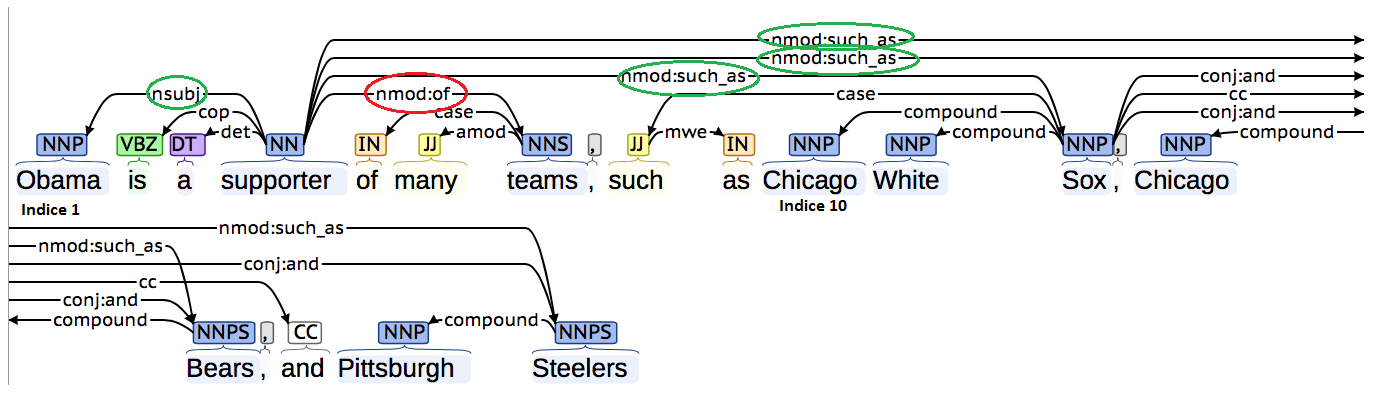
\includegraphics[width=\textwidth,height=6cm]{figure/dipendenze.png}
  \caption{Nella figura vengono mostrate le dipendenze individuate tramite la libreria di Stanford. Gli nmod rilevanti, cerchiati in verde, sono quelli che presentano diversi dependent. nmod:of viene quindi scartato in quanto presenta una sola dependent.}
\end{figure*}
 Essenzialmente si adotta questo processo perch\'e le dependent di ciascun nmod rappresentano le possibili liste di entit\'a contenute nella sequenza di fatti che si vuole estrarre. \\La fase successiva consiste nell'individuazione del soggetto del sottoperiodo in esame. Si procede quindi con la navigazione delle dipendenze a partire dal governor comune degli nmod, cercando il ramo che porta alla dipendenza \textit{nsubj}. Il dependent di nsubj \'e proprio il soggetto del sottoperiodo.
\\A questo punto del processamento sostanzialmente sono state individuate le entit\'a coinvolte nel fatto da estrarre, il passo successivo consiste dunque nel riuscire a localizzare la frase caratterizzante il fatto stesso. 
\\Vengono quindi richiesti gli indici corrispondenti al soggetto e alla prima entit\'a coinvolta nella lista. Tali indici corrispondono alla posizione della parola all'interno della frase. \\Prendendo in considerazione l'esempio fornito nella Figura 6 avremmo che gli indici in questione sono 1, quello di ``Obama'', e 10, ``Chicago''. \\Presa la frase delimitata dagli indici individuati si prosegue con il Pos Tagging, eseguito ancora dalla libreria di Stanford. L'obiettivo di questa fase \'e l'individuazione dei verbi e delle congiunzioni subordinate\footnote{http://www.ling.upenn.edu/courses/Fall\_2003/ling001/penn\_treebank\_pos.html}. \\ Queste operazioni sono risultate particolarmente rilevanti perch\'e le frasi individuate vengono poi state utilizzate per la ricerca di nuovi fatti. \\I principali problemi riscontrati sono i seguenti:
\begin{enumerate}
\item prendere tutta la frase compresa tra gli indici, escludendo magari soltanto i list identifiers, come ad esempio ``such as'' o ``like'', compromette la possibilit\'a di generalizzare la frase. \\Poich\'e le frasi estratte vengono successivamente passate al filtro relazionale si rischierebbe di perdere tutte le frasi eccessivamente lunghe.
\item prendere soltanto il verbo all'interno del periodo rischia invece di stravolgerne il significato, con la possibilit\'a concreta di inserire fatti sbagliati nel knowledge graph.
\end{enumerate}
Abbiamo quindi cercato dei compromessi tra queste soluzioni opposte andando ad includere anche le preposizioni e le congiunzioni subordinate presenti tra il verbo e la  prima entit\'a della lista. Con riferimento ancora alla Figura 6 otterremmo come output: \textit{\\ 
 Obama is a supporter of Chicago White Sox\\
 Obama is a supporter of Chigago Bears\\ 
 Obama is a supporter of Pittsburgh Steelers}\\
Su questo tipo di frasi elementari e ben definite i risultati sono pi\'u che soddisfacenti, tuttavia all'aumentare della complessit\'a del periodo, l'output peggiora sensibilmente. In particolare, si verifica spesso che la frase estratta ha un significato diverso o parziale rispetto a quella originale. Al termine del processamento le frasi estratte vengono quindi passate al filtro relazionale, per poi seguire il processo di estrazione di fatti presentato in precedenza.
I tempi di esecuzione di questa componente sono risultati estremamente lunghi e per questo \'e senza dubbio necessario scalare orizzontalmente, splittando il file ed eseguendo il calcolo di dipendenze su pi\'u calcolatori. Anche la valutazione del processo di estrazione di fatti da frase lista, di conseguenza, \'e stata effettuata su un campione di \textbf{10.000} frasi passate alla libreria di Stanford.

\section{Valutazione dei fatti estratti}
Al termine del processo di implementazione abbiamo quindi valutato i fatti estratti mediante tecniche diverse:
\begin{enumerate}
\item fatti estratti senza generalizzazione di frasi e senza preprocessamento
\item fatti estratti mediante generalizzazione
\item fatti estratti mediante generalizzazione e stopping
\item fatti estratti dalle frasi lista
\end{enumerate}
Abbiamo quindi preso in considerazione le medesime relazioni usate per la valutazione dei nuovi fatti estratti su FreeBase, impostando inoltre la probabilit\'a minima di \textit{0.5} e \textit{K=20}. Per la tecnica di estrazione senza preprocessamento abbiamo valutato 470 fatti, per quelle basate sul preprocessamento 240 ciascuna e per l'analisi delle frasi lista circa 280.  Abbiamo inoltre adottato una soluzione di crowdsourcing, rivolgendoci a quattro nostri colleghi. Il costo di tale operazione \'e stato quantificato  in un caff\'e ogni 80 fatti valutati. Sebbene, paragonando il carico di lavoro e il costo relativo alle offerte presenti su Amazon Mechanical Turk ci siamo accorti che la ricompensa era troppo elevata, abbiamo comunque accettato il compromesso, trattandosi di persone qualificate.



\begin{table*}[h]
\vspace*{-65pt}
\centering
\caption{In tabella i risultati ottenuti applicando Lector su \textbf{FreeBase}}
\begin{center}
\label{table_ASME}
\begin{tabular}{c c c c c}
& & \\ % put some space after the caption
\hline
Relazione & \# Fatti in FreeBase & \# nuovi fatti & \# fatti valutati & \# accuratezza \\
\hline
birthPlace &  \textit{662.192} &   \textit{57.140}  &  \textit{347} &  \textit{88,9\%} \\
deathPlace &\textit{178.849} &   \textit{18.458} &  \textit{104} & \textit{80,6\%} \\
nationality & \textit{584.792} &   \textit{50.234} &  \textit{290} & \textit{95,6\%} \\
team & \textit{145.080} &   \textit{49.809}  &  \textit{286} & \textit{96,5\%} \\
almaMater & \textit{378.043} &   \textit{46.342}  &   \textit{286} & \textit{98,3\%} \\
spouse & \textit{130.425} &   \textit{14.939} &  \textit{97} & \textit{31,6\%} \\
child & \textit{141.860} &   \textit{3.149}  &  \textit{50} & \textit{38,8\%} \\
award & \textit{98.625} &   \textit{1.934}  &  \textit{50} & \textit{96,4\%} \\
party &\textit{65.300} &   \textit{3.684}  &  \textit{50}  & \textit{94,5\%} \\

\hline
\end{tabular}
\end{center}
\end{table*}

\begin{table*}[h]
\vspace*{-145pt}
\centering
\caption{In tabella i risultati ottenuti applicando Lector su \textbf{YAGO} senza generalizzazione e stopping}
\begin{center}
\label{table_ASME}
\begin{tabular}{c c c c c}
& & \\ % put some space after the caption
\hline
Relazione & \# Fatti in YAGO & \# nuovi fatti & \# fatti valutati & \# accuratezza \\
\hline
wasBorn &  \textit{280.942} &   \textit{57.837}  &  \textit{40} &  \textit{90,4\%} \\
diedIn &\textit{94.728} &   \textit{22.203} &  \textit{40} & \textit{81,6\%} \\
isCitizenOf & \textit{36.253} &   \textit{28.763} &  \textit{40} & \textit{96,3\%} \\
playsFor & \textit{525.358} &   \textit{23.716}  &  \textit{40} & \textit{87,9\%} \\
graduatedFrom & \textit{51.478} &   \textit{50.229}  &   \textit{40} & \textit{96,3\%} \\
isMarriedTo & \textit{34.219} &   \textit{16.119} &  \textit{40} & \textit{35,1\%} \\
hasChild & \textit{42.330} &   \textit{14.617}  &  \textit{40} & \textit{25,4\%} \\
hasWonPrize & \textit{120.465} &   \textit{25.736}  &  \textit{50} & \textit{93,1\%} \\
isPoliticianOf &\textit{32.774} &   \textit{630}  &  \textit{50}  & \textit{82,5\%} \\
actedIn &\textit{126.236} &   \textit{2.385}  &  \textit{50}  & \textit{96,7\%} \\
\hline
\textbf{Totale fatti estratti ( contando tutte le relazioni)} & &  \textit{493.279}  &    &  \\




\end{tabular}
\end{center}
\end{table*}




%´'´`΄՛՝‘‛
%%%%%%%%%%%%%%%%%%%%%%%%%%%%%%%%%%%%%%%%%%%%%%%%%%%%%%%%%%%%%%%%%%%%%%
% The bibliography is stored in an external database file
% in the BibTeX format (file_name.bib).  The bibliography is
% created by the following command and it will appear in this
% position in the document. You may, of course, create your
% own bibliography by using thebibliography environment as in
%
% \begin{thebibliography}{12}
% ...
% \bibitem{itemreference} D. E. Knudsen.
% {\em 1966 World Bnus Almanac.}
% {Permafrost Press, Novosibirsk.}
% ...
% \end{thebibliography}

% Here's where you specify the bibliography style file.
% The full file name for the bibliography style file 
% used for an ASME paper is asmems4.bst.



\end{document}
